\documentclass[11pt,a4paper,titlepage,oneside]{report}
\usepackage{titling}
\usepackage{graphicx}
\usepackage{mathtools}
\usepackage{lmodern}
\usepackage{amsmath}
\usepackage{float}
\usepackage{subfig}
\usepackage{listings}

%% Memoir layout setup

%% NOTE: You are strongly advised not to change any of them unless you
%% know what you are doing.  These settings strongly interact in the
%% final look of the document.

% Dependencies
\usepackage{bfhlogo}
\usepackage{etoolbox}% http://ctan.org/pkg/etoolbox

\makeatletter
%%begin novalidate
%% Titlepage adjustments
\pretitle{\vspace{0pt plus 0.7fill}\begin{center}\Huge}
\posttitle{\end{center}\par}
\preauthor{\par\begin{center}\let\and\\\Large}
\postauthor{\end{center}}
\predate{\par\begin{center}\Large}
\postdate{\end{center}}
%%end novalidate
\def\@advisors{}
\newcommand{\advisors}[1]{\def\@advisors{#1}}
\def\@department{}
\newcommand{\department}[1]{\def\@department{#1}}
\def\@thesistype{}
\newcommand{\thesistype}[1]{\def\@thesistype{#1}}

\renewcommand{\maketitlehooka}{\noindent\bfhlogo[2cm]}

\renewcommand{\maketitlehookb}{\vspace{1in}%
  \par\begin{center}\Large\sffamily\@thesistype\end{center}}

\renewcommand{\maketitlehookd}{%
  \vfill\par
  \begin{flushright}
    \sffamily
    \@advisors\par
    \@department, BFH
  \end{flushright}
}

% Fix the chapters (unnecessary space)
\patchcmd{\@makechapterhead}{\vspace*{50\p@}}{}{}{}% Removes space above \chapter head
\patchcmd{\@makeschapterhead}{\vspace*{50\p@}}{}{}{}% Removes space above \chapter* head

\makeatother

\setlength{\droptitle}{-48pt}


\title{Point cloud-based camera calibration}
\author{Stefan Eichenberger}
\date{August 2018}
\advisors{Marcus Hudritsch}
\department{HuCE CPVR Lab}

\begin{document}
\maketitle

\begin{abstract}
To reconstruct the pose and position of a camera the intrinsic camera model must once be calculated. We show a method on how to calibrate a camera based on a pregenerated point cloud. This method makes camera calibration more user friendly for augmented reality applications where pregenerated point clouds can be used.
\end{abstract}

\tableofcontents

\chapter{Introduction}
In 1865 the Christoffeltower in Bern was destroyed to create space for a new railway station. In a today's point of view this decision was a mistake. They destroyed a part of history back then.\\
Today the area around the railway station is heavily used by buses and cars. Therefore, it is impossible to reconstruct the tower physically. Luckily we nowadays have the technology to at least create the illusion of such a building. The idea is to create a virtual Chritoffeltower by using augmented reality on a smartphone.\\\\
One problem of this idea is that we don't know what kind of device a possible viewer will use. Therefore it is not possible to use calibration data of a predefined camera type. It must be possible to calibrate the camera right in place. This is where this project comes in. The goal is to calibrate a camera based on a pregenerated point cloud.

\section{Camera Calibration}\label{sec:calibration}
Camera calibration is necessary to find a model that expresses the properties of the camera. Properties of a camera can be defined as follows:
\begin{itemize}
	\item Focal length of the objective
	\item Principal point on the camera sensor where the z axis goes trough
	\item Distortion of the objective
	\item Size of a pixel
\end{itemize}
If we once know the camera model as well as the camera position we are able to project virtual objects into a real world image. Figure \ref{fig:model} shows an image of a checkerboard where we project a virtual cube onto. One camera model in this image took distortion into account while the other one ignored it.
\begin{figure}[H]
  \begin{center}
		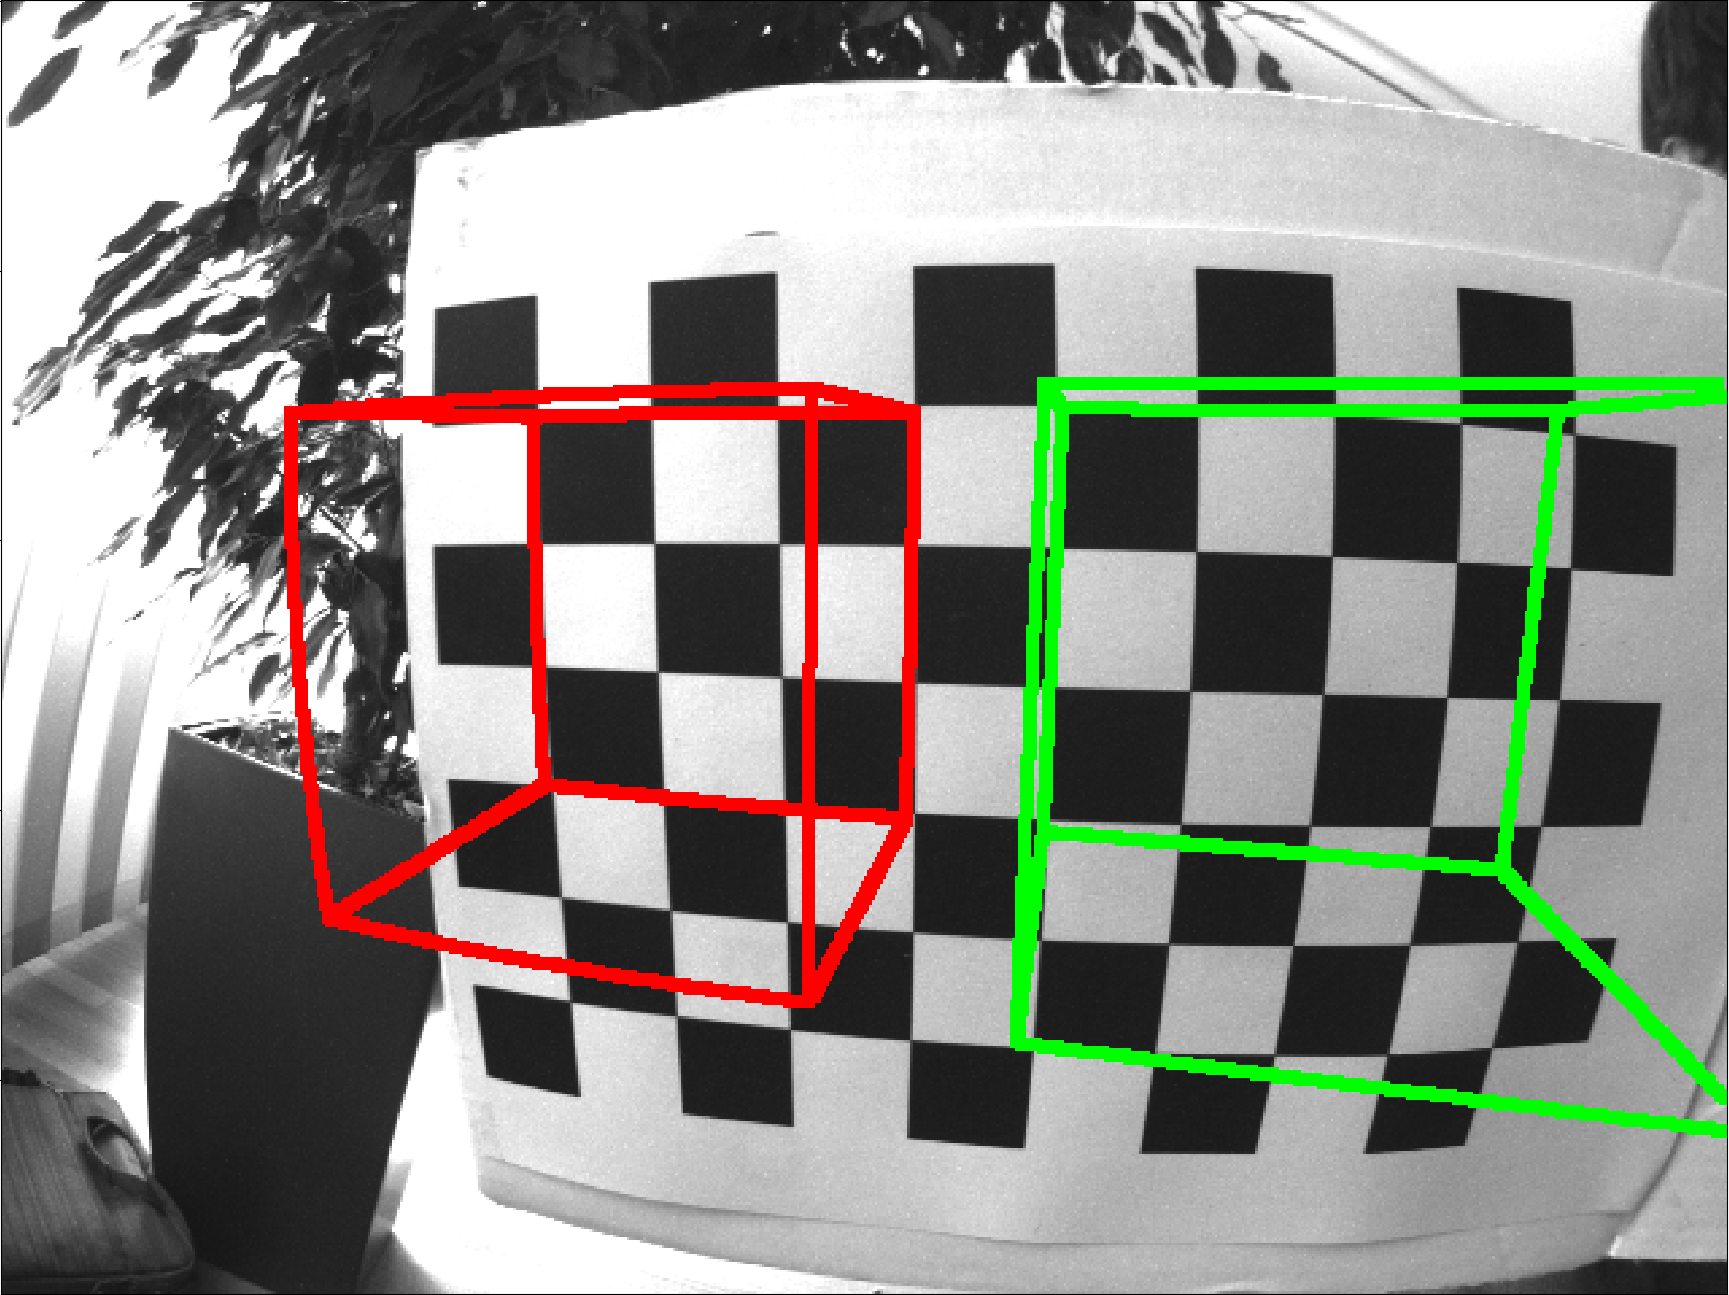
\includegraphics[width=1.0\textwidth]{img/model.png}
  \end{center}
	\caption{Applied camera model with (left) and without(right) distortion}\label{fig:model}
\end{figure}

\section{Goals}
A program should be written that takes a 3D point cloud and 2d points as inputs and calculates the camera model. The tasks for this project are:
\begin{itemize}
\item Search for existing solution
\item Get used to the topic SLAM, AR and 3D representation
\item Choose a programming environment (Python, Matlab)
\item Implement a proof of concept with synthetic data
\item Implement a proof of concept with real world data
\end{itemize}

\chapter{Evaluation}

As a first task some existing solution to similar problems were studied and different tools were analyzed to gain an overview about the topic.

\section{Existing methods}
\subsection{Checkerboard}\label{sec:checkerboard}
The most famous variant for camera calibration is the checkerboard approach \cite{Zhang}. For this approach one must take photos of a checkerboard. The algorithm then performs the following tasks:
\begin{enumerate}
  \item Search the checkerboard corners
  \item Find an approximation of the extrinsic matrix
  \item Find an approximation of the intrinsic matrix
  \item Solve the non linear camera model by minimizing the reprojection error with levenberg-marquart
\end{enumerate}

\subsection{Self-calibration with planar scene}
In comparison to the checkerboard calibration this approach doesn't need a checkerboard. It uses the same technique as checkerboard calibration but instead of using a known image any planar image can be used for calibration \cite{selfcalib}. The algorithm tries to estimate the camera model by doing a bundle adjustment over several images. In comparison to the checkerboard calibration this is more computational expensive and requires more images for doing the calibration.

\subsection{Decision}
Because the Checkerboard calibration is widely used and well documented, this method has been chosen for this project. We don't have a checkerboard available but a 3D cloud instead. The self calibrating approach would be interesting as well but it wouldn't profit from the 3D point cloud. Further it requires a planar image which we can not guarantee to be available when doing calibration. As we will see in chapter \ref{chap:implementation} our method needs some modification to the checkerboard calibration to allow calibration based on 3D points.

\section{Tools}
\subsection{Matlab}
Matlab does have a powerful imaging toolbox. Besides that Matlab also has a lot of powerful tools to plot images, graphs etc. Matlab is a proprietary product of Mathworks. Matlab is available for all mayor operating systems.

\subsection{Python}
Python does not provide as much powerful tools out of the box as Matlab. However, trough additional libraries it can become as powerful as Matlab. Python is developed as open source software and is available for all mayor operating systems.\\
The following additional libraries are required to provide similar functionalities as Matlab:
\begin{itemize}
  \item Scipy
    \subitem Adds some missing mathematically functions like Levenberg-Marquardt or linear least squares
  \item Numpy
    \subitem Is a verry powerful framework for handling matrices
  \item OpenCV
		\subitem Adds image processing and computer vision (CV) features
  \item Matplotlib
    \subitem Adds some powerful visualisation tool
  \item VisVis
    \subitem Allows GPU accelerated visualisation in Python
\end{itemize}

\subsection{Decision}
Because Python has a fast growing community and because we can use OpenCV as CV-toolkit, the decision was made to use Python as programing language. It should be easy to port code written in Python/OpenCV to C++/OpenCV if required.

\chapter{Implementation}\label{chap:implementation}
\section{Optimization}
What we will see later is that an optimization algorithm is required to fit a model to an actual camera. We will use two different kind of optimization algorithms. One is linear least squares which is an optimization algorithm that minimises linear mean squares problems linearly. The second algorithm we will use is Levenberg-Marquardt which is used to solves nonlinear least squares problems. This chapter describes the differences of this algorithms as well as which algorithm should be used for which problem.

\subsection{Linear least squares}
Assume you have a problem in the form show in equation \ref{eq:least_squares_example1}.
\begin{equation}\label{eq:least_squares_example1}
  A*X=B \\ 
  \begin{pmatrix}
    a_{11} a_{12} \\
    a_{21} a_{22}
  \end{pmatrix}*
  \begin{pmatrix}
    x_1 \\
    x_2
  \end{pmatrix}=
  \begin{pmatrix}
    b_1 \\
    b_2
  \end{pmatrix}
\end{equation}
Where:
\begin{align*}
  a		  &: \text{known input values}\\
  x	  	&: \text{unkonwns}\\
  b		  &: \text{known output values}
\end{align*}
We try to find x. This is easy doable by inverting Matrix A and multiply the inverse with B. This will give us the unknown matrix X. We assume here that the matrix is non singular. Let us now assume we have more equations than unknowns which is a common use case in reality. We will then have something like in \ref{eq:least_squares_example2}. This example isn't solvable by inverting matrix A. Instead we need a new algorithm called linear least squares \ref{eq:least_squares_algorithm}. This algorithm tries to minimize the squared error of the equation. For more details on why this algorithm works see \cite{Monson}. Libraries that implement this kind of algorithms are often able to do a pseudo inverse instead of a simple inverse in case that a matrix is non singular. Such an implementation is e.g. pinv of Numpy \cite{pinv}.
\begin{equation}\label{eq:least_squares_example2}
  A*X=B \\ 
  \begin{pmatrix}
    a_{11} a_{12} \\
    a_{21} a_{22} \\
    a_{31} a_{32} \\
    a_{41} a_{42}
  \end{pmatrix}*
  \begin{pmatrix}
    x_1 \\
    x_2
  \end{pmatrix}=
  \begin{pmatrix}
    b_1 \\
    b_2 \\
    b_3 \\
    b_4
  \end{pmatrix}
\end{equation}

\begin{equation}\label{eq:least_squares_algorithm}
  X=(A^H*A)^{-1}*A^H*B 
\end{equation}

An advantage of using a linear solver for the least squares problem is that it will find the global minimum. It is also computationally faster for problems with low to medium amount of unknowns (1-1000). However as the name states it can only solve problems where the unknowns are linear.

\subsection{Gradient-Descent}
Non-linear problems are much harder to solve. Algorithms for this kind of problem can't guarantee to find the global optimum if the problems are non-convex. One of the most common non-linear solvers is gradient descent. Gradient descent is an iterative algorithm which calculates the gradient at point x and then takes a step in the opposite direction of the gradient for minimizing a problem (see Figure \ref{fig:gradient_descent}). The update formula for gradient descent is shown in equation \ref{eq:gradient_descent}.
\begin{figure}[H]
  \begin{center}
    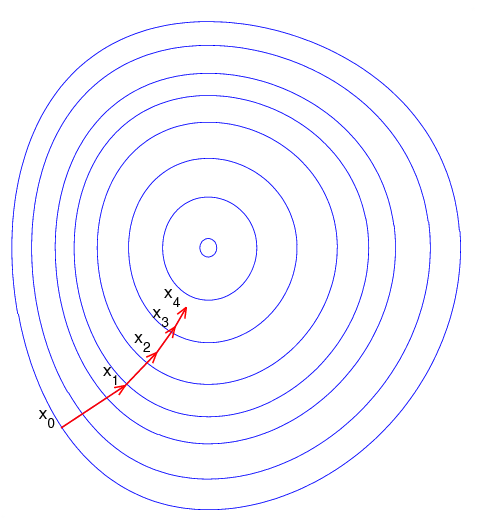
\includegraphics[width=0.5\textwidth]{img/gradient_descent.png}
  \end{center}
    \caption{Gradient descent}\label{fig:gradient_descent}
\end{figure}

\begin{equation}\label{eq:gradient_descent}
  x_{n+1}=x_n-\theta*\Delta f(x_n)
\end{equation}
Where:
\begin{align*}
  x		      &: \text{Parameters}\\
  \Delta f  &: \text{Derivation of function f to optimize}\\
  \theta    &: \text{Step size}
\end{align*}

Gradient-Decent is simple to implement and works well on most non-linear optimization problems.

\subsection{Gauss-Newton}
The Newton optimization algorithm is an algorithm that assumes a problem is approximately quadratic near the optimal solution. It does also derivate the function at a specific location but it will then jump immediately to the position where the derivation is zero (Figure \ref{fig:newton}a). If the problem is quadratic near the optimal solution this algorithm converges faster than gradient descent.

\begin{figure}[H]
	\centering
	\subfloat[Principle \cite{newton_image}]{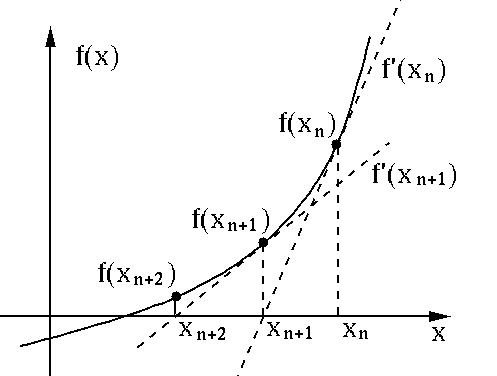
\includegraphics[width=0.4\textwidth]{img/newton.png}}
	\qquad
	\subfloat[Not converging in step 3]{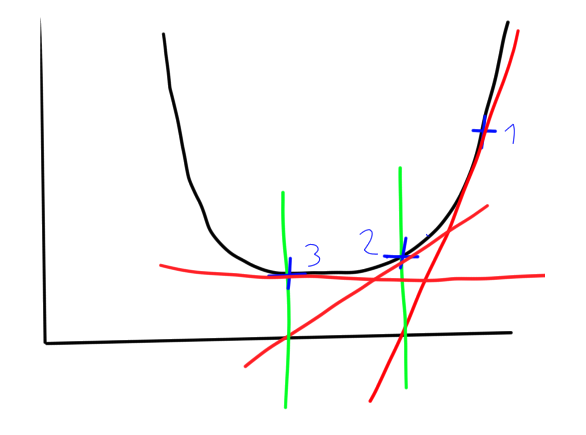
\includegraphics[width=0.4\textwidth]{img/gn_converge.png}}
	\caption{Newton algorithm}
	\label{fig:newton}
\end{figure}

Gauss-Newton on the other hand only works to minimize a sum of squared values while classic Newton works on all problems. However, Gauss-Newton has the advantage of being computational faster \cite{gauss_newton} because it doesn't need to compute the Hessian matrix. The update formula to solve for Gauss-Newton is shown in equation \ref{eq:gauss_newton}.

\begin{equation}\label{eq:gauss_newton}
  x_{n+1} = x_n - (J_n^T*J_n)^{-1}*J_n*e_n
\end{equation}
Where:
\begin{align*}
  x		  &: \text{Parameters to tune}\\
  n		  &: \text{Step}\\
	J		  &: \text{Jacobian matrix \cite{Jacobian}}\\
  e  	  &: \text{The error y-ŷ}
\end{align*}

Newton/Gauss-Newton is not guaranteed to converge if the problem is not approximately quadratic near the optimal solution as shown in Figure \ref{fig:newton}b. In this image the problem is nearly linear near the optimal solution.

\subsection{Levenberg-Marquardt}
For this project Levenberg-Marquardt was chosen as non-linear optimization algorithm. This has been proposed by Zhang who first described the checkerboard calibration \cite{Zhang}. Levenberg-Marquardt uses Gauss-Newton which makes it fast to converge but can move to gradient descent if Gauss-Newton isn't converging. This makes Levenberg-Marquardt more robust than Gauss-Newton but makes it faster than gradient descent. Equation \ref{eq:levenberg_marquardt} shows the update equation for the parameters. \mu\ is the tuning parameter which will increase the influence of gradient descent. If \mu\ is very small (close to 0) then only Gauss-Newton is used. If \mu is huge then only gradient descent is used for optimization. \mu\ can be updated during optimization. If the error increases from step to step, the influence of gradient descent must be increased because Gauss-Newton would never find the optimal solution.

\begin{equation}\label{eq:levenberg_marquardt}
  x_{n+1} = x_n - (J_n^T*J_n + \mu*I)^{-1}*J_n*e_n
\end{equation}
Where:
\begin{align*}
  x		  &: \text{Parameters to tune}\\
  n		  &: \text{Step}\\
  J		  &: \text{Jacobian}\\
  \mu	  &: \text{Learning coefficient for gradient descent}\\
  I     &: \text{Identity matrix}\\
  e  	  &: \text{The error y-ŷ}
\end{align*}

\section{Camera model}
The camera model expresses how any point in the 3D space can be projected onto a two dimensional image. As a first approximation it is assumed that all rays are going trough one point. This is called the pinhole camera model \ref{fig:projection}a. With this assumption the projection of point in 3 dimensional space onto a two dimensional image can be formulated as shown in equation \ref{eq:cm}. 
\begin{equation}\label{eq:cm}
  \begin{pmatrix}fx & \gamma & cx \\
      0 & fy & cy \\
      0 & 0 & 1 \\
    \end{pmatrix}*
    \begin{pmatrix}
      r_{00} & r_{01} & r_{02} & tx \\
      r_{10} & r_{11} & r_{12} & ty \\
      r_{20} & r_{21} & r_{22} & tz \\
    \end{pmatrix}
    \begin{pmatrix}
      X \\
      Y \\
      Z \\
      1
    \end{pmatrix}=
    \begin{pmatrix}
      u \\
      v \\
      s
  \end{pmatrix}
\end{equation}
Where:
\begin{align*}
  X,Y,Z		&: \text{point in the 3D world}\\
  u,v	    	&: \text{point in a 2d image}\\
  s		&: \text{scaling factor (1 when normalized)}\\
	fx,fy   	&: \text{focal length of the camera}\\
  cx,cy   	&: \text{principal point}\\
  tx,ty,tz	&: \text{location of the camera}\\
  r_{ij}	&: \text{part of the rotation matrix}
\end{align*}

We can explain this as follows. A Point (X,Y,Z) is projected onto an image sensor (u,v) by the multiplication of an intrinsic times an extrinsic matrix. The extrinsic matrix describes how the pinhole of the camera is located in the three dimensional space. The intrinsic matrix describes how the camera itself is constructed. For example in figure \ref{fig:projection}b a point $p_i$ is rotated and translated by the extrinsic matrix so that it's coordinates are described with the pinhole as origin. The point is then further transformed by the intrinsic camera matrix onto the image sensor.\\
\em
Note:\\
In chapter \ref{sec:cam_calib} we said that the pixel size must also be known. This is true but will not appear directly in the camera model. The parameters fx and fy who normally are sizes in meters are expressed in pixels. They therefore include the information about pixel size.
\normalfont

\begin{figure}[H]
	\centering
	\subfloat[Pinhole model]{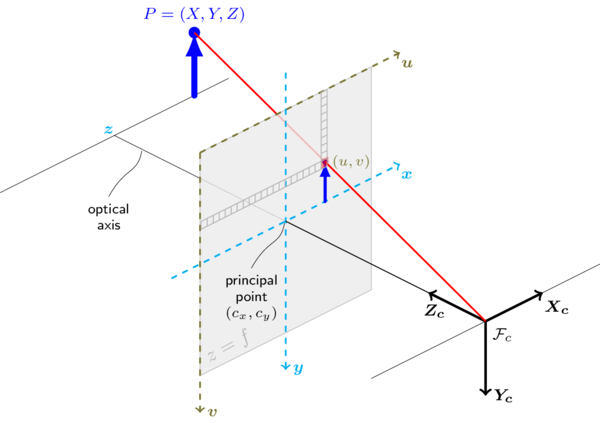
\includegraphics[width=0.5\textwidth]{img/pinhole_camera_model.png}}
	\subfloat[3D point to 2D point]{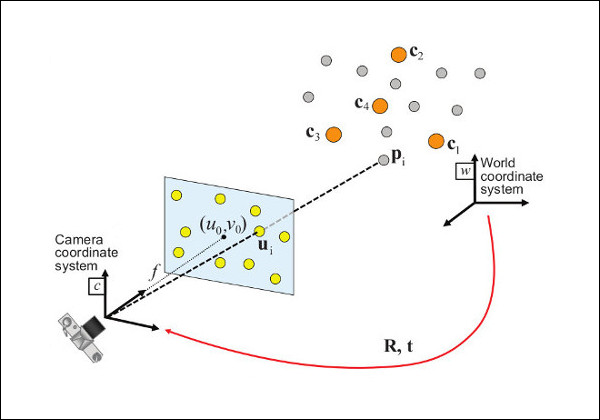
\includegraphics[width=0.5\textwidth]{img/pnp.jpg}}
	\caption{Image projection}\label{fig:projection}
\end{figure}

When calibrating a camera we are interested in the intrinsic matrix because it will be constant over time for a specific camera. Additional to the intrinsic matrix a real world objective will have distortion. This means an image is not mapped perfectly onto the image plane. It is non linear distorted the further a pixel is placed from the principal point (cx,cy). How distortion affects the image is shown in equation \ref{eq:dist}.

\begin{equation}\label{eq:dist}
	\begin{pmatrix}\gamma_{u} \\
	  \gamma_{v}
	\end{pmatrix}=\begin{pmatrix}
	  u(k_1r^2+k_2r^4+k_3r^6)\\
	  v(k_1r^2+k_2r^4+k_3r^6)
	\end{pmatrix}+\begin{pmatrix}
	  2p_1uv+p_2(r^2+2u^2)\\
	  p_1(r^2+2v^2)+2p_2uv
	\end{pmatrix}
\end{equation}
\begin{equation}\label{eq:pdist}
\begin{pmatrix}u'\\v'\end{pmatrix}=\begin{pmatrix}
u\\v\end{pmatrix}+\begin{pmatrix}\gamma_{u}\\\gamma_{v}\end{pmatrix}
\end{equation}
Where:
\begin{align*}
  k_{i}		&: \text{radial distortion}\\
  p_{i}	    	&: \text{tangential distortion}\\
  \gamma_{i}	&: \text{summed distortion}\\
  u',v'		&: \text{distorted image points}
\end{align*}

By doing camera calibration we try to find a model which maps the 3D points onto a 2D image. The image calculated by the model must be as close as possible to the real image. This fitting the model to reality is a non-linear optimization task. What makes it non-linear is the distortion which depends on the position of the pixel in the image. How we can optimize this model we will see in the next sections

\section{Camera calibration}\label{sec:cam_calib}
This section describes how the camera model is used to calibrate the camera in different steps.

\subsection{Estimate the projection matrix}\label{sec:est_proj}
Non-linear optimization can only find local optimum. Therefore we require a good initial guess of where we start with optimization. Because the distortion is not huge, an initial guess can be done with linear optimization. For this we assume the camera model does not have any distortion. We need to find the $c_{ij}$ values in equation \ref{eq:projection}. The projection matrix C (containing $c_{nn}$) is a multiplication of the intrinsic times the extrinsic matrix. The assumption that the distortion is small only holds for regular objectives but not for fisheye objectives. We are focusing on regular onces for this project.

\begin{equation}\label{eq:projection}
	\begin{pmatrix}c_{11} & c_{12} & c_{13} & c_{14}\\
		c_{21} & c_{22} & c_{23} & c_{24}\\
		c_{31} & c_{32} & c_{33} & c_{34}\\
	\end{pmatrix}*
	\begin{pmatrix}
		X \\
		Y \\
		Z \\
		1
	\end{pmatrix}=
	\begin{pmatrix}
		u \\
		v \\
		s
  \end{pmatrix}
\end{equation}
Where:
\begin{align*}
	c_{ij}		&: \text{Unknown camera projection values of projection matrix C}\\
	X,Y,Z			&: \text{3D Point}\\
	u,v,s			&: \text{2D Point}\\
\end{align*}

We can rewrite equation \ref{eq:projection} as shown in equation \ref{eq:projection_flat}. We don't know u and v directly. We only have the pixel position which is $x=u/s, y=v/s, 1$. There is no way to estimate s. We know that s equals to the third row of equation \ref{eq:projection_flat}. If we multiply x and y by the third row the equation will still hold (equation \ref{eq:projection_flat_s}. As a side effect we can remove the third row because the left and right side are equal which always holds. We finally have two equation per image point. Another trick we use is to set $c_{34}$ to 1. This makes the Z position of the camera the norm for the X and Y position (proof by solving intrinsic*extrinsic matrix). With this change the trivial solution where every unknown is zero disappears. The final equation \ref{eq:projection_flat_red} can be solved for all unknowns $c_{ij}$ by linear least squared.

% Make sure we can have the whole column matrix (normally a line break will follow after 10 columns)
\setcounter{MaxMatrixCols}{15}
\begin{equation}\label{eq:projection_flat}
	\begin{pmatrix}
		X & Y & Z & 1 & 0 & 0 & 0 & 0 & 0 & 0 & 0 & 0\\
		0 & 0 & 0 & 0 & X & Y & Z & 1 & 0 & 0 & 0 & 0\\
		0 & 0 & 0 & 0 & 0 & 0 & 0 & 0 & X & Y & Z & 1\\
	\end{pmatrix}
	\begin{pmatrix}c_{00}\\
		c_{11}\\
		c_{12}\\
		c_{13}\\
		c_{14}\\
		c_{21}\\
		c_{22}\\
		c_{22}\\
		c_{23}\\
		c_{31}\\
		c_{32}\\
		c_{33}\\
		c_{34} \\
	\end{pmatrix}=
	\begin{pmatrix}u\\
		v\\
		s\\
	\end{pmatrix}
\end{equation}

\begin{equation}\label{eq:projection_flat_s}
	\begin{pmatrix}u\\
		v\\
		s\\
	\end{pmatrix}\\=
	\begin{pmatrix}x*(X*c_{31}+Y*c_{32}+Z*c_{33}+c_{34})\\
		y*(X*c_{31}+Y*c_{32}+Z*c_{33}+c_{34})\\
		1*(X*c_{31}+Y*c_{32}+Z*c_{33}+c_{34})\\
	\end{pmatrix}
\end{equation}


\begin{equation}\label{eq:projection_flat_red}
	\begin{pmatrix}
		X & Y & Z & 1 & 0 & 0 & 0 & 0 & -uX & -uY & -uZ\\
		0 & 0 & 0 & 0 & X & Y & Z & 1 & -vX & -vY & -vZ
	\end{pmatrix}
	\begin{pmatrix}
		c'_{00}\\
		c'_{11}\\
		c'_{12}\\
		c'_{13}\\
		c'_{14}\\
		c'_{21}\\
		c'_{22}\\
		c'_{23}\\
		c'_{24}\\
		c'_{31}\\
		c'_{32}\\
		c'_{33}
	\end{pmatrix}=
	\begin{pmatrix}x\\
		y\\
	\end{pmatrix}
\end{equation}
Where:
\begin{align*}
	c_{ij}		&: \text{unknown camera projection values}\\
	c'_{ij}		&: \text{same as c but normalized to $c_{34}$}\\
	X,Y,Z			&: \text{3D Point}\\
	u,v,s			&: \text{2D Point with scale factor s}\\
	x,y				&: \text{2D Point normalize to s=1}\\
\end{align*}

One last step is missing, we set $c_{34}$ to 1 to get rid of the trivial solution where all $c_{ij}$ are zero. We now have to try to find the right value for $c_{34}$. If we calculate the intrinsic times extrinsic we end up in equation \ref{eq:ext_int}. We focus on the third row. We know that the norm of a column of a rotation matrix must be one. The reason for this is that a rotation matrix will never change the length of a vector. Therefore $h=\sqrt{r_{31}^2+r_{32}^2+r_{33}^2}$ must be one \cite{Wu}. Because we normalized tz to one, this assumption wont hold for our solution. The camera distance $t_z$ will therefore be $1*1/h$. To correct the whole projection matrix we can multiply the whole matrix with $1/h$ (equation \ref{eq:ext_int_scaled}).

\begin{equation}\label{eq:ext_int}
	C=
	\begin{pmatrix}
		f_xr_{11}+c_xr_{31} & f_xr_{12}+c_xr_{32} & f_xr_{13}+c_xr_{33} & f_xt_x+c_xt_z\\
		f_yr_{21}+c_yr_{31} & f_yr_{22}+c_yr_{32} & f_yr_{23}+c_yr_{33} & f_yt_y+c_yt_z\\
		r_{31} & r_{32} & r_{33} & t_z
	\end{pmatrix}
\end{equation}

\begin{equation}\label{eq:ext_int_scaled}
	C=1/h
	\begin{pmatrix}
		c'_{11} & c'_{12} & c'_{13} & c_{14}\\
		c'_{21} & c'_{22} & c'_{23} & c_{24}\\
		c'_{31} & c'_{32} & c'_{33} & 1\\
	\end{pmatrix}
\end{equation}

Where:
\begin{align*}
	C					&: \text{projection matrix}\\
	C'				&: \text{projection matrix found with $t_z=1$}\\
	f_x,f_y		&: \text{focal length}\\
	c_x,c_y		&: \text{principal point}\\
	r_{ij}		&: \text{Parameters of rotation matrix}\\
	t_{x,y,z}	&: \text{location of the camera}\\
	h					&: \text{real $tz=1/\sqrt{r_{31}^{'2}+r_{32}^{'2}+r_{33}^{'2}}$}
\end{align*}


After the unknowns are found we have have a first approximation of the projection matrix. In the next step we need to decompose this projection matrix into the intrinsic and extrinsic matrix.\\
\em
Note:\\
This equation is the same for checkerboard calibration. In comparison we need to find all 11 unknowns where for checkerboard calibration $c_{n2}$ doesn't appear \cite{Zhang}. The reason is that for checkerboard calibration all Z values are set to zero. This is due to the planar property of a checkerboard. Because Z is zero, $c_{n2}$ can be anything it wont affect the final result. In our case we have a 3D point cloud therefore Z will not necessarily be zero and we have to take it into account.
\normalfont

\subsection{Matrix decomposition}\label{sec:matrix_dec}
If we take a closer look at the intrinsic camera matrix we see that this matrix has the form shown in \ref{eq:uptriang}. This is called an upper triangular matrix.
\begin{equation}\label{eq:uptriang}
	\begin{pmatrix}
		a_{00} & a_{01} & a_{02}\\
		0 & a_{11} & a_{12}\\
		0 & 0 & a_{22}
	\end{pmatrix}
\end{equation}

We can decompose any rectangular matrix into an orthogonal matrix times an upper triangular matrix with a RQ-decomposition \cite{qr_decomposition}. Most mathematic libraries don't offer the RQ-decomposition but a QR-decomposition which are relatives. In this project the following algorithm for QR/RQ convertion was used \cite{rq_stack}:
\begin{enumerate}
	\item Compute $A^{*}=P*A$ (Where P = equation \ref{eq:qr_p})
	\item Compute decomposition of $A^{*T}=Q^*R^*$
	\item Set $Q=PQ^{*T}$ (i.e. reverse rows of $Q^{*T}$, note that Q is orthogonal)
	\item Set $R=PR^{*T}P$
\end{enumerate}

\begin{equation}\label{eq:qr_p}
	P=\begin{pmatrix}
		0 & 0 & 1\\
		0 & 1 & 0\\
		1 & 0 & 0
	\end{pmatrix}
\end{equation}
\em
Note:\\
There is an additional parameter $a_{01}$ which we don't use in the camera model. In theory this value should converge to zero. In reality this value will be small but more than zero. For non-linear estimation we set $a_{01}$ to zero. Non-linear optimization will later correct this error.
\normalfont

\subsection{Non-Linear estimation}\label{sec:nonlinear_est}
Until now we ignored the non-linear distortion. We took a simple linear model and optimized it to find the intrinsic camera matrix. This matrix can be used as initial guess for optimizing the non-liner model. For the non-linear optimization we calculate the reprojection error of each point as shown in equation \ref{eq:reprojecterr}.
\begin{equation}\label{eq:reprojecterr}
	e=\sum\limits_{i=1}^n(u_{should}-u_{is})^2 +(v_{should}-v_{is})^2
\end{equation}
In some resource we can find that it is possible to calculate a first guess for the distortion parameters with a linear model as well. In theory this is true with equation \ref{eq:distortion_lin}.  However because the intrinsic and extrinsic camera matrix are already an approximation the linear least squared solution for the distortion will be completely wrong and this approach is not suitable. Instead, a good initial estimation of the distortion parameters is to assume all unknowns are zero. The reason why zero is a good guess is that we already assumed that they are zero while doing linear optimization. After that we can optimize the whole camera model with Levenberg-Marquardt by minimizing the reprojection error of equation \ref{eq:reprojecterr}.

\begin{equation}\label{eq:distortion_lin}
	\begin{pmatrix}
		f_x\\
		f_y
	\end{pmatrix}.*
	\begin{pmatrix}
		xr^2 & xr^4 & xr^6 & 2xy & r^2+2x^2 \\
		yr^2 & yr^4 & yr^6 & r^2+2y^2 & 2xy
	\end{pmatrix}
	\begin{pmatrix}
		k1\\k2\\k3\\p1\\p2
	\end{pmatrix}=
	\begin{pmatrix}
		u_{should}-u_{est}\\
		v_{should}-v_{est}
	\end{pmatrix}
\end{equation}
Where:
\begin{align*}
  f_x/f_y		&: \text{focal length}\\
	x,y				&: \text{Position on the sensor measured from principal point}\\
	r					&: \text{Radius measured from principal point}\\
	k1,k2,k3	&: \text{Radial distortion}\\
	p1,p2			&: \text{Tangential distortion}\\
	.*				&: \text{Element wise matrix multiplication}
\end{align*}

\subsection{Outlier Detection}\label{sec:outliers}
The described approach so far works well if there are no outliers in the dataset. This is true for synthetic data but not for real world data. Therefore an algorithm is needed to detect outliers. For this project an algorithm similar to RANSAC \cite{ransac} is used. Instead of calculating the projection matrix \ref{eq:projection} once, the calculation is done iteratively with a reduced and randomized dataset. The estimation that fits the data best will be used for further calculations. Outliers that have a huge reprojection error will be removed from the dataset.
\begin{enumerate}
	\item Get a random subset of 10 data points
	\item Calculate the projection matrix as shown in equation \ref{eq:projection_flat}
	\item Estimate the projection points based on the estimated camera model
	\item Calculate the distance of each point to where it should be
	\item Count the points as hit where the point is within a radius of 3px
	\item Repeat steps 1-5 n times, take the model with the most hits
	\item Remove all points that do not count as hit from the dataset
\end{enumerate}

In this project n was chosen to be 1000 for synthetic data and 2000 for real world data.

\subsection{Final algorithm}
The final algorithm performs the following steps:
\begin{enumerate}
	\item Take a randomized reduced set of data from all data
	\item Calculate the projection matrix with linear least squares \ref{sec:est_proj}
	\item Calculate the projection of each point
	\item Detect outliers \ref{sec:outliers}
	\item Repeat steps 1-4 n times
	\item Do matrix decomposition \ref{sec:matrix_dec} to find intrinsic matrix
	\item Do non-linear estimation \ref{sec:nonlinear_est} to optimize the whole model with distortion
\end{enumerate}

The final output will be the intrinsic matrix and the five distortion parameters $k_i$ + $p_i$.

\section{Point cloud}
So far we ignored how we get to 3D and 2D points for estimating the camera model. This two steps are not part of this project, however they were needed to generate a real world example. This section gives a small overview on how a 3D point cloud can be generated.\\
A point cloud is a collection of points within a 3-dimensional space. We know the position (x,y,z) of each point and its unique descriptor. The descriptor must be translation and rotation invariant. The cloud can be stored in a file or database for future use. We chose ORB2 monocular SLAM \cite{orbslam2} to generate this cloud because it is open source, good documented and well established. Monocular SLAM is chosen because its handling is much simpler than with other systems (e.g. stereo camera). ORB2 Slam performs simplified the following steps:
\begin{enumerate}
\item Search distinctive points on the image e.g. corners
\item Calculate an ORB descriptor at all distinctive points
\item Calculate the translation and rotation between two views
\item Calculate the position and rotation of the camera in the local coordinate system
\item Calculate the position of the points
\end{enumerate}
We store the position and the ORB descriptor of each point in a file to make the point cloud persistent.
In theory, our approach needs 6 points to solve equation \ref{eq:cm} with 17 unknowns. To solve equation \ref{eq:dist} another 5 unknowns are added. In theory, we would need 8 points in total. In practice, more points are required to detect outliers and to reduce the influence of noise. Trough trial and error an estimate of around 20 points is well suited to solve our problem. More points will of course work as well and can reduce the influence of noise.\\
This projects goal wasn't to generate a point cloud therefore we don't explain the algorithm and steps in more detail here. In theory any type of point cloud could be used as long as the 3D points can be matched against 2d points somehow.

\chapter{Result}
\section{Proof of concept}
A proof of concept was made that allows testing the algorithm with synthetic data. With this proof of concept we are able to simulate noise and outliers to see how the algorithm performs. Because we know the exact camera parameters we can calculate the distance from the estimated values to the real values at the end. The difference of the image calculated with the real model an with the estimated model can be shown in an image like Figure \ref{fig:diff_img}. To make have a difference visible white noise needs to be added to the image data before doing the estimation. Without noise the estimated model matches the real model good enough to not show any differences.
\begin{figure}[H]
  \begin{center}
		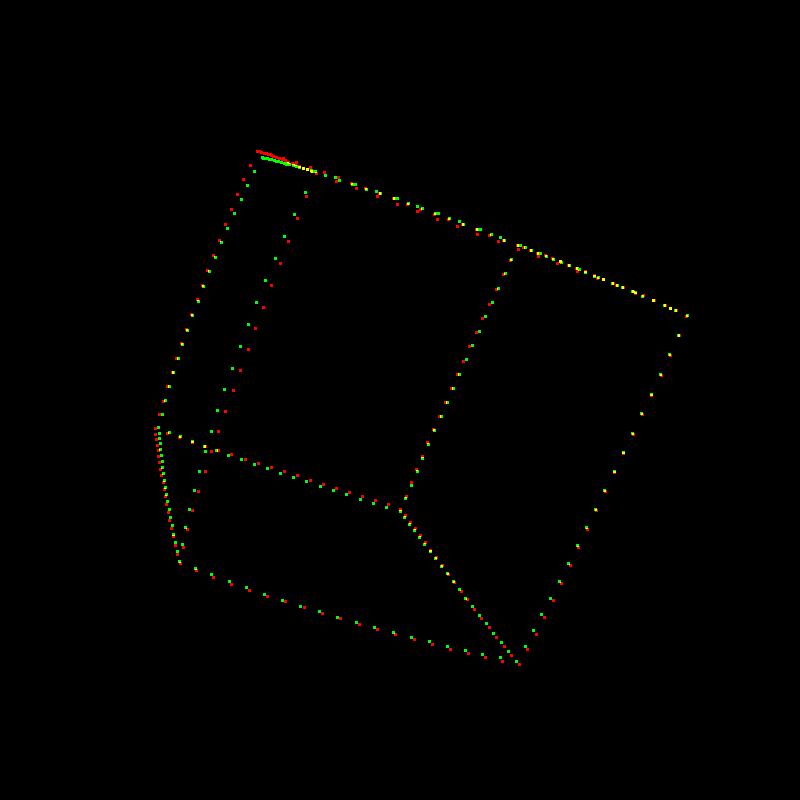
\includegraphics[width=1.0\textwidth]{img/diff_img.png}
  \end{center}
	\caption{Comparison real (green) with estimated (red) model when image data is noisy}\label{fig:diff_img}
\end{figure}

\section{Real data}
To show that the proof of concept works an example application was written that takes an image and a pointcloud as input and will then calibrate the camera based on that information. The application performes the following steps:
\begin{enumerate}
	\item Search ORB keypoints on the image
	\item Calculate ORB descriptor around each keypoint
	\item Match ORB descriptors with descriptors found in the point cloud with BFMatcher \cite{BFMatcher} based on Hamming distance
	\item Generate pairs of 3D and 2d points based on matches from the previous step
	\item Start camera calibration as described in section \ref{sec:cam_calib}
\end{enumerate}
For generating a point cloud we modified the ORB2\_SLAM open source implementation \cite{orbslam2_impl} to allow exporting 3D points as well as the corresponding descriptors. It is also possible to use SLProject from the CPVR lab to generate the 3D point cloud.

An example output of camera-calibration.py which is part of this project is shown here:
\tiny
\begin{lstlisting}
Start camera calibration
Extract descriptors
Match keypoints
Optimize camera model
Found camera parameters:
        fx      fy      cx      cy      thetax  thetay  thetaz  tx      ty      tz      k1      k2      k3      p1      p2
values: 1318.89 1320.44 646.11  361.73  0.04    0.01    0.03    0.01    -0.0    -0.01   0.35    -2.78   8.12    -0.01   0.0
Exit program
\end{lstlisting}
Values from checkerboard calibration for the same camera:
\begin{lstlisting}
        fx      fy      cx      cy      k1      k2      k3      p1      p2
values: 1333    1333    629     362     0.31    -2.37   6.65    -0.0003 0.0002
\end{lstlisting}
This gives us an uncertainty per parameter of:
\begin{lstlisting}
        fx      fy      cx      cy      k1      k2      k3      p1      p2
diff:   1.05%   0.94%   2.72%   0.07%   12.90%  17.30%  12.32%  32.33% 100%
\end{lstlisting}
\normalsize
Besides the small values who only have a small influence, the calibration works well. This uncertainties are there because of noise and inaccuracy in the point cloud. However, the camera model would work well for augmented reality. An example of an undistorted image with this parameters can be seen in figure \ref{fig:undistorted}.

\begin{figure}[H]
  \begin{center}
		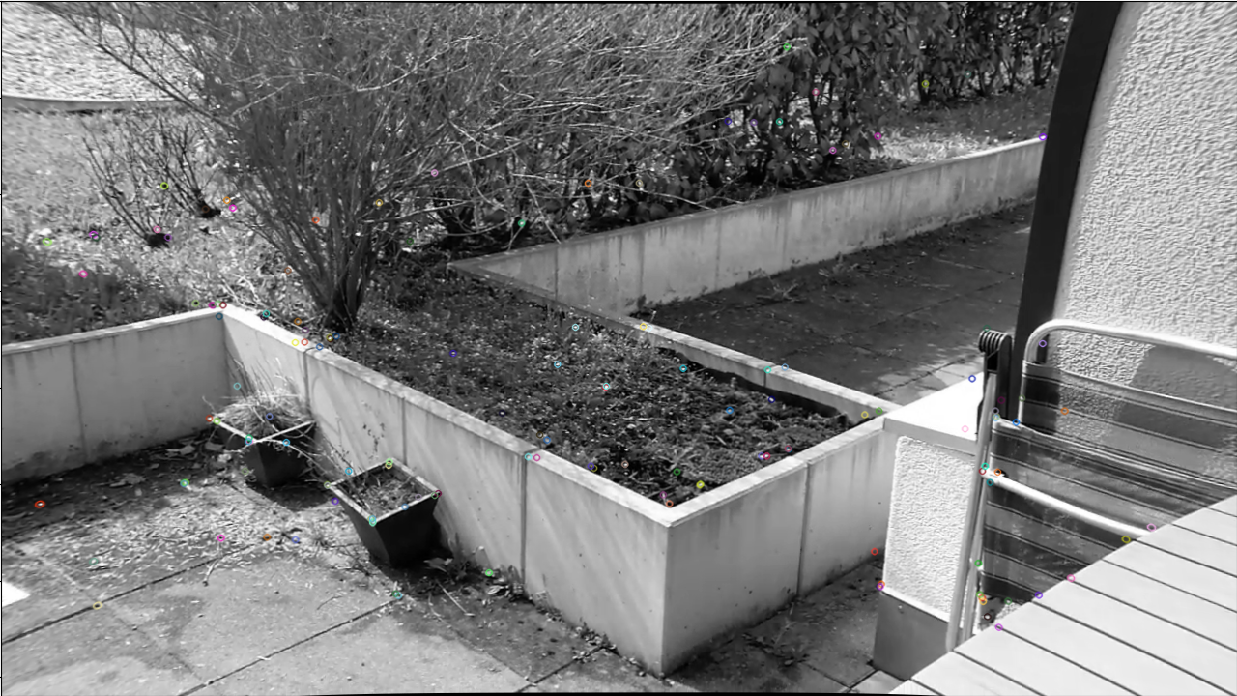
\includegraphics[width=1.0\textwidth]{img/calib_output.png}
  \end{center}
	\caption{Undistorted image after calibration with colored keypoints}\label{fig:undistorted}
\end{figure}

\section{Improvements}\label{sec:improvements}
The algorithm described in this document only shows the calibration process on a single image. This works well but isn't very robust. OpenCV in comparison uses several images for doing checkerboard calibration. With this approach it can detect when the non linear optimization goes in wrong directions. OpenCV also does bundle adjustment over several images which reduces the influence of noise and increases the robustness. This methods could be used to improve our algorithm as well and make it more robust against noise, outliers and converging into wrong solutions.

\begin{thebibliography}{1}

  \bibitem{surf}
  Herbert Bay1, Tinne Tuytelaars2, and Luc Van Gool,
  \textit{SURF: Speeded Up Robust Features}
  http://www.vision.ee.ethz.ch/~surf/eccv06.pdf (09.07.2018)

  \bibitem{orbslam}
  Raul Mur-Artal, J. M. M. Montiel, Juan D. Tardos
  \textit{ORB-SLAM: a Versatile and Accurate Monocular SLAM System}
  arXiv:1502.00956v2

  \bibitem{orbslam2}
  Raul Mur-Artal, J. M. M. Montiel, Juan D. Tardos
  \textit{ORB-SLAM2: an Open-Source SLAM System for Monocular, Stereo and RGB-D Cameras}
	arXiv:1610.06475v2 

  \bibitem{orbslam2_impl}
  Raul Mur-Artal, J. M. M. Montiel, Juan D. Tardos
  \textit{ORB-SLAM2 Implemenation}
	https://github.com/raulmur/ORB\_SLAM2


  \bibitem{selfcalib}
  Daniel Herrera et al.
  \textit{Forget the checkerboard: practical self-calibration using a planar scene}
  doi:10.1109/WACV.2016.7477641

  \bibitem{Hayes}
  Monson H. Hayes,
  \textit{Statistical Digital Signal Processing And Modeling},
  Wiley, ISBN 0-47159431-8

  \bibitem{pinv}
  Numpy,
  \textit{scipy.linalg.pinv},
  Compute the (Moore-Penrose) pseudo-inverse of a matrix

  \bibitem{gauss_newton}
  Wikipedia,
  \textit{Gauss-Newton algorithm},
  https://en.wikipedia.org/wiki/Gauss\%E2\%80\%93Newton\_algorithm (08.07.2018)

  \bibitem{newton_image}
  http://fourier.eng.hmc.edu,
  \textit{Newton Ralphson Method}
  http://fourier.eng.hmc.edu/e176/lectures/NM/node20.html (09.07.2018)

  \bibitem{Zhang}
  Zhengyou Zhang,
  \textit{A Flexible New Technique for Camera Calibration}
  MSR-TR-98-71

	\bibitem{qr_decomposition}
	William H. Press,
	\textit{Numerical Recipes 3rd Edition: The Art of Scientific Computing, p102-109} 
	Cambridge University Press, ISBN 0-52188068-8

	\bibitem{rq_stack}
	johnnycrab,
	\textit{rq-decomposition} 
	https://math.stackexchange.com/questions/1640695/rq-decomposition (10.07.2018)

	\bibitem{ransac}
	wikipedia,
	\textit{RANSAC}
	https://de.wikipedia.org/wiki/RANSAC-Algorithmus

	\bibitem{BFMatcher}
	OpenCV,
	\textit{Brute-force descriptor matcher}
	https://docs.opencv.org/3.1.0/d3/da1/classcv\_1\_1BFMatcher.html

	\bibitem{Jacobian}
	Wikipedia,
	\textit{Jacobian matrix}
	https://en.wikipedia.org/wiki/Jacobian\_matrix\_and\_determinant

	\bibitem{Wu}
	Ying Wu,
	\textit{Image Formation and Camera Calibration}
	http://users.eecs.northwestern.edu/~yingwu/teaching/EECS432/Notes/camera.pdf (19.08.2018), Electrical Engineering \& Computer Science Northwestern University Evanston

\end{thebibliography}


\end{document}
